\subsection{Singularity Detection Monitor} \label{ssec:Singularitaeten}
Im Folgenden wird der Singularity Detection Monitor zur Erkennung von
singulären Gelenkpositionen des Roboters näher erläutert. Ziel ist es,
Handgelenks-, Ellbogen- und Schulter-Singularitäten festzustellen und beim
Auftreten Events mit relevanten Informationen wie Achswinkeln, Nähe zur
Singularität sowie verbleibende Manipulierbarkeit des Roboters auszugeben.

\subsubsection{Theoretische Grundlagen der Singularitätsdetektion}
\label{sssec:Theorie_Singularitaeten}
Kinematische Singularitäten stellen ein fundamentales Problem in der
Robotersteuerung dar und treten auf, wenn die Jacobi-Matrix des Roboters ihren
vollen Rang verliert. In diesen Konfigurationen verliert der Roboter die
Fähigkeit, sich in bestimmte Richtungen im kartesischen Raum zu bewegen, was zu
Kontrollverlust und potentiell gefährlichen Situationen führen
kann.\vglcite{siciliano2016robotics}

Eine kinematische Singularität tritt auf,
wenn die Jacobi-Matrix $\mathbf{J}(\boldsymbol{\theta})$, welche des Roboters
ihren vollen Rang verliert:
\begin{equation}
  \text{rank}(\mathbf{J}(\boldsymbol{\theta})) < \min(m, n)
  \label{eq:singularity_condition}
\end{equation} wobei
$\mathbf{J}(\boldsymbol{\theta}) \in \mathbb{R}^{m \times n}$ die Jacobi-Matrix,
$\boldsymbol{\theta}$ der Gelenkwinkelvektor, $m$ die Anzahl der Freiheitsgrade
im kartesischen Raum und $n$ die Anzahl der Robotergelenke darstellt.
\noindent
Die Jacobi-Matrix beschreibt die Beziehung zwischen Gelenkgeschwindigkeiten
$\dot{\boldsymbol{\theta}}$ und kartesischen Geschwindigkeiten des TCP
$\mathbf{v}$:
\begin{equation} \mathbf{v} = \mathbf{J}(\boldsymbol{\theta})
  \dot{\boldsymbol{\theta}} \label{eq:jacobian_velocity}
\end{equation}
\noindent
Tritt eine Singularität auf, so wird die Jacobi-Matrix singulär.
\begin{equation} \det(\mathbf{J}) = 0 \label{eq:jacobian_singularity}
\end{equation} Dadurch wird die inverse Kinematik nicht
eindeutig lösbar ist und es können theoretisch unendliche
Gelenkgeschwindigkeiten auftreten.\vglcite{nakamura1991advanced}

\subsubsection{Frameworkspezifisches Vorgehen}
Im Rahmen der praktischen Implementierung wird hier ein auf Schwellwerten und
absoluten sowie winkelbasierten Entfernungen zur Singularität angewendet. Durch
die Anwendung der rein mathematischen Definition ließe sich zwar jede beliebige
Singularität in einer seriellen Kinematik erkennen, jedoch bleiben die
betroffenen Gelenke und Art der Singularität ungewiss und müssten iterativ
bestimmt werden. Daher wird hier eine pragmatische Berechnungsmethodik
verwendet.

Für serielle Robotermanipulatoren mit sechs Freiheitsgraden, wie den hier
verwendeten ABB IRB 6700, können drei primäre Singularitätstypen unterschieden
werden: Schultersingularitäten, Ellbogensingularitäten und
Handgelenksingularitäten.\vglcite{spong2006robot}

\paragraph{Schultersingularitäten} treten auf, wenn sich das
Handgelenkszentrum (Schnittpunkt der Achsen 4, 5, 6) direkt über oder nahe der
Rotationsachse des ersten Gelenks befindet:

\begin{equation}
  \sqrt{x_{wc}^2 + y_{wc}^2} < \epsilon
  \label{eq:shoulder_singularity}
\end{equation}
\noindent
wobei $(x_{wc}, y_{wc})$ die Position des Handgelenkszentrums in der XY-Ebene
und $\epsilon$ der Singularitätsschwellenwert ist.

\paragraph{Ellbogensingularitäten} treten auf, wenn der Roboter die
Grenzen seines
Arbeitsraums erreicht. Dies geschieht typischerweise bei vollständig
ausgestreckter oder eingeklappter Konfiguration. Beim
Knickarmrobotern wie dem IRB 6700
verläuft die Rotationsachse des vierten Gelenks nicht direkt durch
den Ursprung vom
dritten Gelenk, sondern ist durch eine Translation verschoben. Das impliziert,
dass die vollständige Streckung des Armes nicht durch einen Winkel
von $0^\circ$ bzw.
$180^\circ$ auftritt. Hier lässt sich allgemeiner der Zusammenhang der Vektoren
zwischen Gelenk 2 und 3 sowie 2 und 5 anwenden:

\begin{equation}
  \theta = \angle(\vec{v}_{23}, \vec{v}_{25}) \approx 0^\circ \text{
  oder } \theta \approx 180^\circ
  \label{eq:elbow_singularity}
\end{equation}

wobei:
\begin{align}
  \vec{v}_{23} & = \vec{p}_3 - \vec{p}_2 \\
  \vec{v}_{25} & = \vec{p}_5 - \vec{p}_2
\end{align}

mit $\vec{p}_i$ als Position des Gelenks $i$. Die Singularitätsbedingung lautet:
\begin{equation}
  \theta < \epsilon \quad \text{oder} \quad \theta > 180^\circ - \epsilon
\end{equation}

\paragraph{Handgelenksingularitäten} treten auf, wenn die Rotationsachsen der
letzten drei Gelenke (Gelenke 4, 5, 6) kollinear werden. Dies tritt
typischerweise auf, wenn $\theta_5 = 0^\circ$ oder $\theta_5 =
180^\circ$. Mathematisch
beschrieben durch:

\begin{equation}
  \mathbf{z}_4 \parallel \mathbf{z}_6 \text{ oder } |\mathbf{z}_4
  \cdot \mathbf{z}_6| \approx 1
  \label{eq:wrist_singularity}
\end{equation}
\noindent
wobei $\mathbf{z}_i$ die Rotationsachse (Z-Achse) des $i$-ten Gelenks im
Weltkoordinatensystem darstellt. Beispielhaft ist das Auftreten einer
Handgelenkssingularität in Abbildung~\ref{figure:wristSingularity}
in Unity3D.

\paragraph{Manipulierbarkeitsindex (Yoshikawa-Maß)} Der von Yoshikawa
\cite{yoshikawa1985manipulability} eingeführte Manipulierbarkeitsindex ist eine
der am häufigsten verwendeten Metriken:
\begin{equation}
  \mu(\boldsymbol{\theta}) =
  \sqrt{\det(\mathbf{J}(\boldsymbol{\theta})\mathbf{J}^T(\boldsymbol{\theta}))}
  \label{eq:yoshikawa_measure}
\end{equation}

Für quadratische Jacobi-Matrizen vereinfacht sich dies zu:
\begin{equation}
  \mu(\boldsymbol{\theta}) = |\det(\mathbf{J}(\boldsymbol{\theta}))|
  \label{eq:yoshikawa_simplified}
\end{equation}
\noindent
Der Index nimmt Werte zwischen 0 (Singularität) und einem maximalen Wert an,
wobei höhere Werte bessere Manipulierbarkeit indizieren. Die Robotik-Literatur
bietet verschiedene Ansätze zur Behandlung von Singularitäten, die sich in
präventive und reaktive Strategien unterteilen lassen. Um diese in der Praxis
anzuwenden, müssen jedoch teilweise numerische Auswertungen durchgeführt werden,
um Schwellwerte zu erfassen. Daher kommen diese hier nicht zum Einsatz.

Zur zusätzlichen Charakterisierung wird jedoch die Yoshikawa-Manipulierbarkeit
berechnet, da der Wert als Kennzahl für die Nähe zu einer Singularität verwendet
werden kann. Er wird in den Ergebnissen in Kapitel
\ref{sec:singularityauswertung} aufgeführt.

\begin{figure}[H]
  \centering
  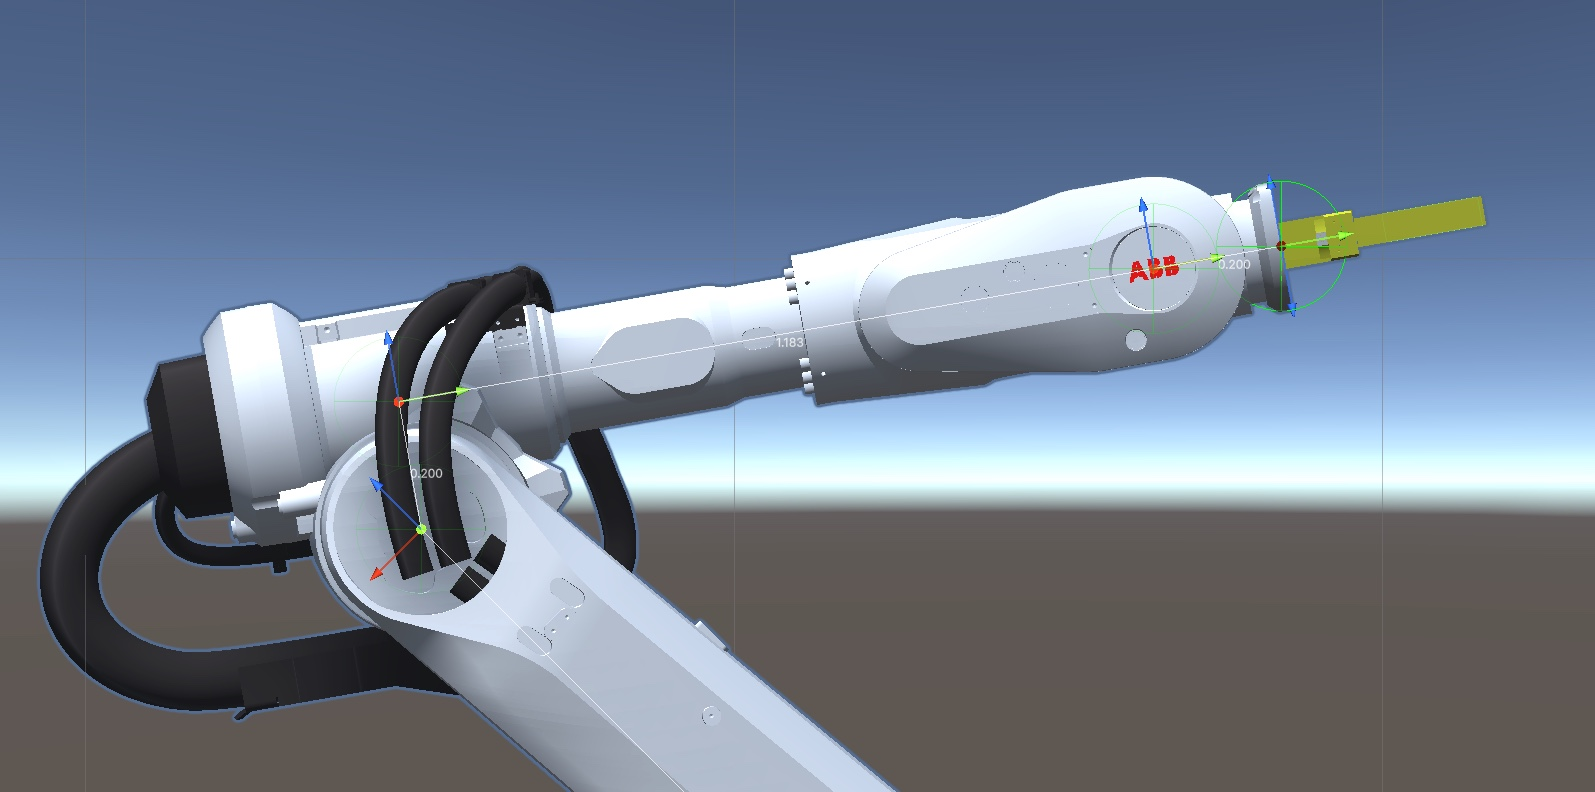
\includegraphics[width=\linewidth]{Figures/wristSingularityScreenshot.jpg}
  \caption{Screenshot einer Handgelenksingularität in Unity mit farbig
  dargestellten Koordinatensystemen der DH-Transformationen}
  \label{figure:wristSingularity}
\end{figure}

\subsubsection{Praktisches Vorgehen} \label{sssec:Framework_Implementierung}
Nachfolgend werden die Schritte 1 bis 4 zur Prüfung des Vorliegens
einer Singularität dargestellt.

\paragraph{Schritt 1: Positionsberechnung und Achsentransformation}~\\
Die Positionen der relevanten Gelenke werden durch die Anwendung der
Vorwärtstransformation nach Denavit-Hartenberg berechnet\vglcite{denavit1955}:
\begin{equation}
  \vec{p}_i = \text{DH}(\theta_1, \ldots, \theta_i) \quad \text{für }
  i = 2, 3, 5
  \label{eq:position_calculation}
\end{equation}
\noindent
Die Rotationsachsen werden aus den Transformationsmatrizen extrahiert:
\begin{equation}
  \mathbf{z}_i = \mathbf{T}_i[:3, 2] \quad \text{für } i = 1, 4, 6
  \label{eq:axis_extraction}
\end{equation}

\paragraph{Schritt 2: Singularitätsanalyse}~\\
Für jeden Singularitätstyp wird die entsprechende Bedingung überprüft:
\begin{itemize}
  \item \textbf{Schultersingularität:}
    \begin{equation}
      d_{wc} = \sqrt{x_{wc}^2 + y_{wc}^2}
    \end{equation}
    wobei $(x_{wc}, y_{wc})$ die Position des Handgelenkszentrums in
    der XY-Ebene ist.

  \item \textbf{Ellbogensingularität:}
    \begin{equation}
      \theta_{elbow} = \angle(\vec{p}_3 - \vec{p}_2, \vec{p}_5 - \vec{p}_2)
    \end{equation}

  \item \textbf{Handgelenksingularität:}
    \begin{equation}
      c_{46} = |\mathbf{z}_4 \cdot \mathbf{z}_6|
    \end{equation}
\end{itemize}

\paragraph{Schritt 3: Schwellwertvergleich}~\\
\begin{table}[H]
  \centering
  \begin{tabular}{l l l}
    \hline
    \textbf{Singularitätstyp} & \textbf{Beispiel-Schwellwert}      &
    \textbf{Bedingung}                            \\
    \hline
    Schulter                  & $\tau_{\text{shoulder}} = 100$ mm  &
    $d_{wc} < \tau_{\text{shoulder}}$             \\
    Ellbogen                  & $\tau_{\text{elbow}} = 5^{^\circ}$ &
    $\theta_{elbow} < \tau_{\text{elbow}}$ oder   \\
    &                                    & $\theta_{elbow} >
    180^\circ - \tau_{\text{elbow}}$ \\
    Handgelenk                & $\tau_{\text{wrist}} = 5^{^\circ}$ &
    $c_{46} > \tau_{\text{wrist}}$                \\
    \hline
  \end{tabular}
  \caption{Singularitätsschwellwerte und Detektionsbedingungen}
  \label{tab:singularity_thresholds}
\end{table}

\paragraph{Schritt 4: Manipulierbarkeitsberechnung}~\\
Für detektierte Singularitäten wird ein approximierter Manipulierbarkeitsindex
nach Yoshikawa berechnet:

\begin{equation}
  w = \sqrt{\det(\mathbf{J}(\theta)\mathbf{J}^T(\theta))}
  \label{eq:manipulability}
\end{equation}
\noindent
Ein kleiner Wert von $w$ indiziert die Nähe zu einer singulären Konfiguration.
Das entwickelte Framework implementiert eine winkelbasierte
Singularitätsdetektion, die geometrische Eigenschaften der Roboterkinematik
direkt nutzt, anstatt auf rechenintensive Jacobi-Matrix-Berechnungen angewiesen
zu sein. Die achsenbasierte Methode basiert auf der Erkenntnis, dass
Handgelenks- und Ellbogensingularitäten geometrisch durch die
Kollinearität von Rotationsachsen
charakterisiert werden können. Schultersingularitäten werden analog durch die
Entfernung des ersten Gelenks zum Handgelenkzentrum in der XY-Ebene
festgestellt.

\subsubsection{Konkrete Implementierung der Detektionsmethoden}
\label{sssec:Implementierung_Detektionsmethoden}
Die Implementierung des \texttt{SingularityDetectionMonitor} nutzt die
Vorwärtskinematik des Preliy Flange Frameworks zur Berechnung der
Gelenkpositionen. Die zentrale Methode \texttt{ComputeJointPosition} berechnet
die kartesische Position eines beliebigen Gelenks durch sukzessive Anwendung
der Denavit-Hartenberg-Transformationsmatrizen (vgl.
Abbildung~\ref{listing:forwardKinematic}).

\begin{figure}[H]
  \inputminted[fontsize=\footnotesize]{csharp}{code-snippets/CalculateJointPos.cs}
  \caption{Vorwärtskinematik zur Positionsberechnung}
  \label{listing:forwardKinematic}
\end{figure}

\noindent
Die Methode \texttt{ComputeJointPosition} in Abbildung
\ref{listing:forwardKinematic} implementiert die klassische
Vorwärtskinematik durch
Multiplikation homogener Transformationsmatrizen. Jede Matrix $\mathbf{T}_i$
wird aus den DH-Parametern $(\alpha_i, a_i, d_i, \theta_i)$ konstruiert, wobei
$\theta_i$ der aktuelle Gelenkwinkel plus einem konstanten Offset ist. Die
resultierende Transformationsmatrix beschreibt die Position und Orientierung des
Gelenks im Basiskoordinatensystem.\\

\noindent
Das Framework nutzt Unitys \texttt{Matrix4x4}-Klasse für die
Transformationsberechnungen und die \texttt{GetPosition()}-Methode zur
Extraktion der Translationskomponente. Die Koordinatentransformation zwischen
dem DH-Parametersystem und Unitys linkshändigem Y-up Koordinatensystem wird
dabei durch die Methode \texttt{HomogeneousMatrix.CreateRaw()} des
Flange-Frameworks transparent gehandhabt. Das ermöglicht eine nahtlose
Integration der mathematischen Robotik-Konzepte in die Unity-Umgebung, während
die Echtzeitfähigkeit durch eventgetriebene Berechnung gewährleistet ist.
Bei der Detektion einer Singularität bzw. dem Unterschreiten des im Unity-Editor
definierten Grenzwertes wird ein \texttt{SafetyEvent}-Objekt
instanziert und an die
\texttt{SafetyMonitor} Klasse weitergegeben. Darin werden zusätzlich
Event-Metadaten zu den
Daten der Gelenkwinkelabstände ausgegeben. Sobald der
kritische Bereich verlassen wurde, wird ein weiteres
\texttt{SafetyEvent} ausgegeben, um
den Bereich, in welcher die Singularität auftritt, abstecken zu können.
